
\documentclass[11pt,letterpaper,oneside]{article}
\usepackage[top=1in,left=1in,right=1in,bottom=1in]{geometry}
\usepackage{fancyvrb}
\usepackage{colortbl}
\usepackage{graphicx}
\usepackage{url}

\title{Checking Inconsistency between Driver code and Document}
\author{Dejun Qian\\Department of Computer Science\\Portland State University\\Portland, OR 97201\\dejun@pdx.edu}

\begin{document}
\maketitle

\begin{abstract}
This report presents how we implement coDoc. 
Experiment result shows that, with our effert in this project, coDoc can provide forthfold, 
1) provide the ability to display code and document. 
2) select code based on syntax parsing.
3) make relationship between code and document.
4) analyze relationship.
\end{abstract}

% Include the motivation for your work, your approach, your goals, and a short summary of what you found/achieved/tested.
\section{Introduction}
\label{sec:introduction}
Verification for software is very important. \cite{xiao_automated_2012}.

The initial version\footnote{\texttt{\url{http://web.cecs.pdx.edu/~cs533acc/arum.git}}} has been released.

The rest of the paper is orgnized as follows. 
Section \ref{sec:methodology} introduce our implementation.
Section \ref{sec:results} gives the experiment result of our implementation. 
Section \ref{sec:conclusion} conclude our work and give some thinking towards the future.

% Explain your design / languages, libraries, and tools used, experimental design.
\section{Methodology}
\label{sec:methodology}
This section presents what we have done and how we did it.

\subsection{Build and Make existing code}
On the first stage of our work, we tried to make the software user-friendly. Basically, the following work is done,
\begin{enumerate}
\item Added Makefile and instructions.
\item Added accurate "usage" message to output.
\end{enumerate}

\begin{figure}
\begin{center}
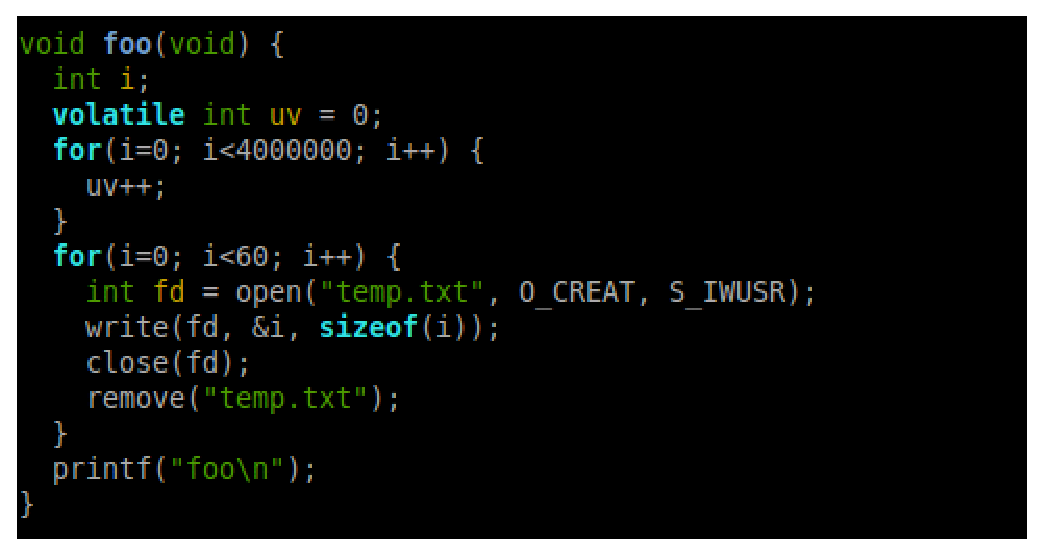
\includegraphics[width=0.6\textwidth]{codoc.eps}
\caption{Structure of Dyninst}
\label{fig:codoc}
\end{center}
\end{figure}

How coDoc works is illustrated in Figure \ref{fig:codoc}\footnote{\texttt{from Bryan's paper \cite{xiao_automated_2012}}}. 
A \emph{point} is a location in a program.

\noindent \newline\textbf{Instrument Using Dyninst}\newline
\indent Figure \ref{fig:codoc} gives a general idea about how coDoc works.

The code used to achieve this goal is shown bellow,
\begin{Verbatim}[frame=single]
printf(``Hello world!'');
\end{Verbatim}


After downloading Elipse\footnote{\texttt{\url{http://www.eclipse.org}}}, we need install JDK.

To test this feature, we designed a test program. 
The functions implemented in the test program is listed in Table \ref{table:functions}.

\begin{table}[th]
\caption{Functions implemented in hello}
\centering
\begin{tabular}{rl}
\hline
Function & Description \\
\hline
fake & functioin never called \\
foo  & basic function \\
recursive & function call itself recursively \\
main & main function \\
\hline
\end{tabular}
\label{table:functions}
\end{table}

% This should NOT be raw data or code listings.  Instead you should present the key results from your work.  Be guided by the papers you have read this quarter - in cases where it is necessary for understanding, a small section of code might be listed, separate from the text, but more commonly an algorithm might be shown.  Results are not long tables of data, rather, one or two graphs, or tables with key rows or columns highlighted or italicized.
\section{Results}
\label{sec:results}
The result for the experiment is shown in fig.


% Based on what you have so far, what can you conclude?  What cool ideas did you think up but not have time to implement so far?
\section{Conclusions and Future Work}
\label{sec:conclusion}
There is still a great deal of opportunity to improve coDoc.


% Follow a standard ACM format for your references.  You have examples in the papers you have read.
\bibliographystyle{acm}
\bibliography{reference}

%\begin{thebibliography}{9}
%\bibitem{bib:coDoc}
%\emph{http://www.coDoc.org}
%\end{thebibliography}

\end{document}
